\chapterimage{Pumping.jpg} % Chapter heading image

\chapter{Pumping Efficiencies and Costs}

% \section{Paragraphs of Text}\index{Paragraphs of Text}


% \everymath{\displaystyle}
% \linespread{2}%controls the spacing between lines. Bigger fractions means crowded lines%
% %\pagestyle{fancy}
% %\usepackage[margin=1 in, top=1in, includefoot]{geometry}
% %\everymath{\displaystyle}
% \linespread{2}%controls the spacing between lines. Bigger fractions means crowded lines%
% %\pagestyle{fancy}
% \pagestyle{fancy}
% \setlength{\headheight}{56.2pt}
% \colorlet{Mycolor1}{green!10!orange!90!}

% \chead{\ifthenelse{\value{page}=1}{
\includegraphics[scale=0.3]{SCC}\\ \textbf \textbf Introduction to Wastewater Treatment}}
% \rhead{\ifthenelse{\value{page}=1}{}{}}
% \lhead{\ifthenelse{\value{page}=1}{}{\textbf Introduction to Wastewater Treatment}}
% \rfoot{\ifthenelse{\value{page}=1}{Module 1: WATR 048 - Spring 2019}{Module 1: WATR 048 - Spring 2019}}

% \cfoot{Page \thepage\ of \pageref{LastPage}}
% \lfoot{Shabbir Basrai}
% \renewcommand{\headrulewidth}{2pt}
% \renewcommand{\footrulewidth}{1pt}

% \newcommand{\stkout}[1]{\ifmmode\text{\sout{\ensuremath{#1}}}\else\sout{#1}\fi}
% %Defining colour with different models.
% \definecolor{mypink1}{rgb}{0.858, 0.188, 0.478}
% \definecolor{mypink2}{RGB}{219, 48, 122}
% \definecolor{mypink3}{cmyk}{0, 0.7808, 0.4429, 0.1412}
% \definecolor{mygray}{gray}{0.6}
% \colorlet{LightRubineRed}{RubineRed!70!}
% \colorlet{Mycolor1}{green!10!orange!90!}
% \definecolor{Mycolor2}{HTML}{00F9DE}

% %New command used in the table with all available colour names
% \newcommand{\thiscolor}[1]{\texttt{#1} \hfill \fcolorbox{black}{#1}{\hspace{2mm}}}

% %This changes the row separation in the table
% \renewcommand{\arraystretch}{1.5}




%\noindent\textsc{Area \& Volume Math Problems}
%\definecolor{shadecolor}{RGB}{200,200,240}
% \item \noindent\textsc{Why Treat Wastewater}




\begin{itemize}
\item Pump is a machine used for moving water (and other fluids) through a piping system and raise the pressure of the water.
\item Pumping is accomplished by transforming the input energy - typically from an electric motor or from other sources such as high-pressure air.
\item The pump calculations in this section are for electrically driven rotodynamic pumps.
\item To move water, a pump will need to overcome resistance due its density, gravitational force and friction.
\item This resistance is dependent on:
\begin{itemize}
\item Height the water needs to be raised.  This height of the fluid in a container is referred to as head. 
\item Quantity of water involved
\end{itemize}
\end{itemize}

\section{Glossary of Pump Calculations Terms}\index{Glossary of Pump Calculations Terms}

\textbf{Force:}  In the English system force and weight are often used in the same way. The weight of the cubic foot of water is $62.4$ pounds. The force exerted on the bottom of the one foot cube is $62.4$ pounds. If we have two cubes stacked on top of one another, the force on the bottom will be $124.8$ pounds.

\textbf{Pressure:} Pressure is a force per unit of area, pounds per square inch or pounds per square foot are common expressions of pressure. 

\textbf{Head:}  Pressure is directly related to the height of a column of fluid. This height is called head or feet of head. Pressure and feet of head head are directly related - \emph{for every one foot of head there is a pressure of $0.433$ psi.}

\vspace{0.2cm}
Thus, $\dfrac{0.433 \enspace psi}{ft \enspace (water \enspace column)}$ or conversely $\dfrac{1 \enspace ft \enspace (water \enspace column)}{2.31 \enspace psi}$\\
\texthl{Note:  This pressure/head will include the height the water pumped and also the head associated with friction losses - energy loss because of the water moving through the pipe and fittings.}\\

\begin{figure}[h]
\begin{tikzpicture}
\path[help lines,step=.2] (0,0) grid (16,6);
\path[help lines,line width=.6pt,step=1] (0,0) grid (16,6);
%\foreach \x in {0,1,2,3,4,5,6,7,8,9,10,11,12,13,14,15,16}
%\node[anchor=north] at (\x,0) {\x};
%\foreach \y in {0,1,2,3,4,5,6}
%\node[anchor=east] at (0,\y) {\y};
\pgfmathsetmacro{\cubex}{3}
\pgfmathsetmacro{\cubey}{3}
\pgfmathsetmacro{\cubez}{3}
\draw(13.5,5,3) -- ++(-\cubex,0,0) -- ++(0,-\cubey,0) -- ++(\cubex,0,0) -- cycle;
\draw(13.5,5,3) -- ++(0,0,-\cubez) -- ++(0,-\cubey,0) -- ++(0,0,\cubez) -- cycle;
\draw(13.5,5,3) -- ++(-\cubex,0,0) -- ++(0,0,-\cubez) -- ++(\cubex,0,0) -- cycle;
\draw (8.7,2.5) node[text width=3cm,align=center]
  {\scriptsize{12"}};
\draw (14.1,3.4) node[text width=3cm,align=center]
  {\scriptsize{12"}};
  \draw (10.9,0.5)node[text width=3cm,align=center]
  {\scriptsize{12"}};
    \draw (2.8,4.8)node[text width=3.8cm,align=left]
  {\small{$Pressure=\dfrac{Force}{Area}$}};
      \draw (2.8,3.1)node[text width=3.8cm,align=left]
  {\small{Pressure exerted by}};
        \draw (2.8,2.8)node[text width=3.8cm,align=left]
  {\small{a 1ft column of water}};
        \draw (5.3,2.9)node[text width=3cm,align=center]
  {\small{$=\dfrac{62.4 \enspace lb}{12 in \enspace x \enspace 12 in}$}};
          \draw (7.3,2.9)node[text width=3cm,align=center]
  {\small{$=0.43 \enspace psi$}};
         \draw (3.45,1.2)node[text width=5cm,align=left]
  {\small{As 1$ft^3$ of water weighs 62.4 lbs}};
\end{tikzpicture}
\end{figure}


The pressure at the bottom of a container is affected only by the height of water in the container and not by the shape or the volume of the container. In the drawing below there are four containers all of different shapes and sizes. The pressure at the bottom of each is the same.

\begin{center}
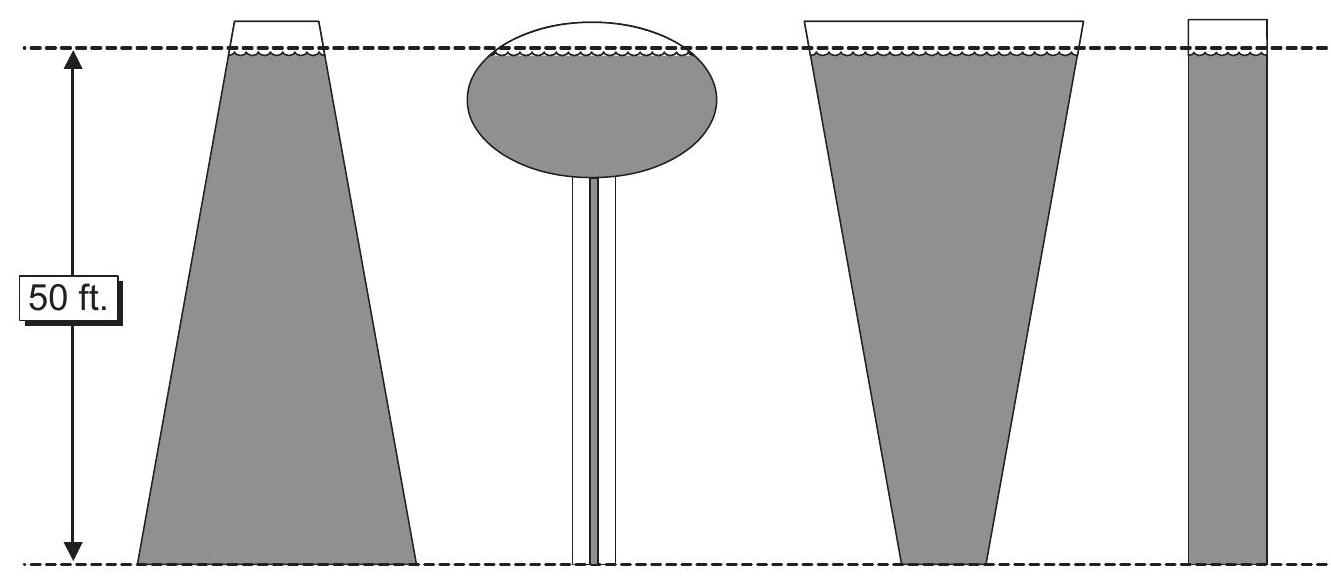
\includegraphics[scale=0.2]{2022_11_03_65aa625ded296bdfd01fg-17}
\end{center}
The pressure exerted at the bottom of a tank is relative only to the head on the tank and not the volume of water in the tank. For example, below are two tanks each containing 5000 gallons. The pressure at the bottom of each is 22 psi. If half of the water were drained from the tanks the pressure at the bottom of the elevated tank would be $17.3$ psi while the pressure at the bottom of the standpipe would be 11 psi.\\

\begin{center}
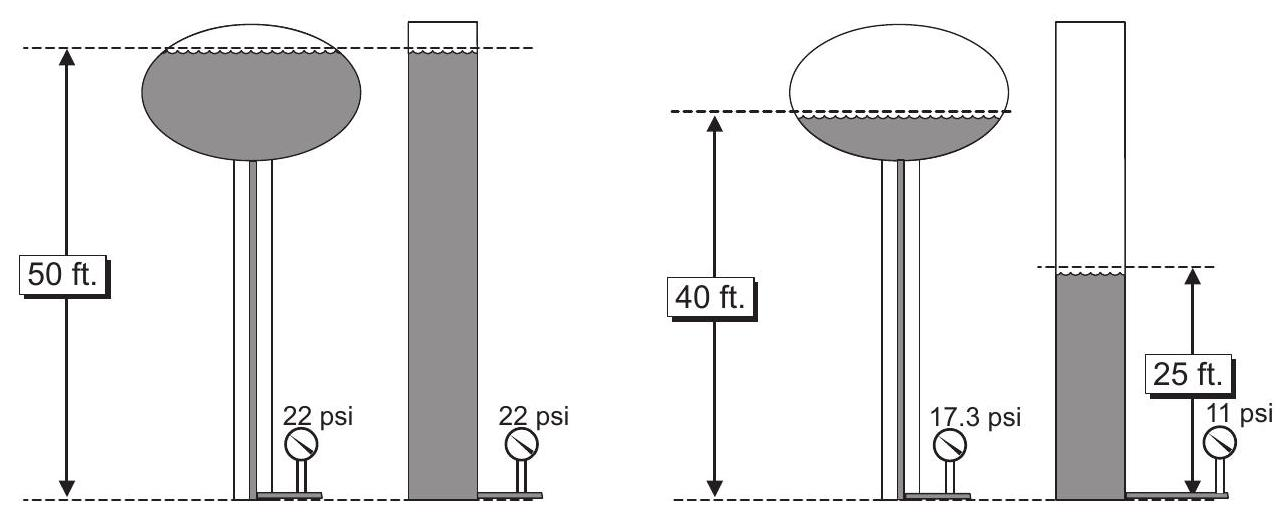
\includegraphics[scale=0.25]{2022_11_03_65aa625ded296bdfd01fg-18}
\end{center}

\textbf{Velocity: } Velocity is the speed that the water is moving along a pipe or through a basin. Velocity is usually expressed in feet per second, $\mathrm{ft} / \mathrm{sec}$.

\textbf{Flow: } Flow is commonly expressed in gallons per minute (gpm) and/or cubic feet per second (cfs). There is a relationship between gallons per minute and cubic feet per second. One cubic foot per second is equal to $448.8$ gallons per minute.

$1 \mathrm{cfs}=448.8 \mathrm{gpm}$

\textbf{Flow Equation; }
The basic equation for determining flow is as follows:

$Q=V \times A$

Where:

$\mathrm{Q}=\operatorname{cfs}\left(\mathrm{ft}^{3} / \mathrm{sec}\right)$

$\mathrm{V}=\mathrm{ft} / \mathrm{sec}$

$\mathrm{A}=\mathrm{ft}^{2}$

\textbf{Static Pressure: } Static implies a non-moving condition.  The pressure measured when there is no water moving in a line or the pump is not running is called static $^{32}$ pressure. This is the pressure represented by the gauges on the tanks in the discussion above.

\textbf{Dynamic Pressure: } When water is allowed to run through a pipe and the pressure (called pressure head) measured at various points along the way we find that the pressure decreases the further we are from the sources.
\begin{center}
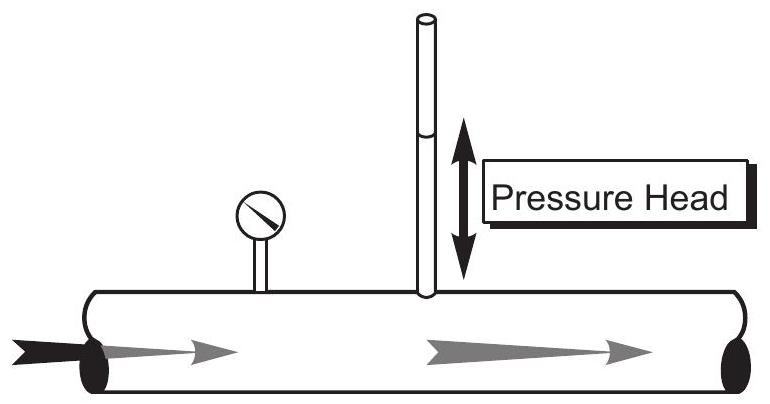
\includegraphics[scale={0.2}]{2022_11_03_65aa625ded296bdfd01fg-18(1)}
\end{center}
\textbf{Headloss: }  The reason for this reduction in pressure is a phenomenon called headloss. Headloss is the loss of energy (pressure) due to friction. The energy is lost as heat.

If the headloss in a certain pipe is 25 feet, it means the amount of energy required to overcome the friction in the pipe is equivalent to the amount of energy that would be required to lift this amount of water straight in the air 25 feet.

In a pipe, the factors that contribute to headloss include the following:

\begin{itemize}
  \item Roughness of pipe - If the roughness of a pipe were doubled the headloss would double.

  \item Length of pipe - If the length of the pipe were doubled the headloss would double.

  \item Diameter of pipe - If the diameter of a pipe were doubled the headloss would be cut in half

  \item Velocity of water - If the velocity of the water in a pipe were doubled the headloss would be increased by about four times. It should be apparent that velocity, more than any other single factor, affects headloss. To double the velocity we would have to double the flow in the line.
  
  \item Pumping System Components and Fittings - Each type of fitting has a specific headloss depending upon the velocity of water through the fitting. For instance the headloss though a check valve is two and one quarter times greater than through a ninety degree elbow and ten times greater than the headloss through an open gate valve.

\end{itemize}

\textbf{Static Head: }  Static head is the distance between the suction and discharge water levels when the pump is shut off. 

\textbf{Suction Lift: } Suction lift is the distance between the suction water level and the center of the pump impeller. This term is only used when the pump is in a suction lift condition. A pump is said to be in a suction lift condition any time the eye (center) of the impeller is above the water being pumped.

\textbf{Velocity Head: } The amount of energy required to bring a fluid from standstill to its velocity. For a given quantity of flow, the velocity head will vary indirectly with the pipe diameter.

\textbf{Total Dynamic Head (TDH):}  The total energy needed to move water from the center line of a pump (eye of the first impeller of a lineshaft turbine) to some given elevation or to develop some given pressure. This includes the static head, velocity head and the headloss due to friction. 

\textbf{Horsepower: } Horsepower is a measurement of the amount of energy required to do work. Motors are rated in horsepower. The horsepower of an electric motor is called brake horsepower. The horsepower requirements of a pump are dependent on the flow and the total dynamic head.  33,000 foot pounds per minute of work is 1 horsepower.

\textbf{Suction Head: } Suction head is the distance between the suction water level and the center of the pump impeller when the pump is in a suction head condition. A pump is said to be in a suction head condition any time the eye (center) of the impeller is below the water level being pumped.

\textbf{Velocity Head: } Velocity head is the amount of energy required by the pump and motor to overcome inertia and bring the water up to speed. Velocity head is often shown mathematically as $\mathrm{V}^{2} / 2 \mathrm{~g}$. ( $\mathrm{g}$ is the acceleration due to gravity $-32.2 \mathrm{ft} / \mathrm{sec}^{2}$ ).
\begin{center}
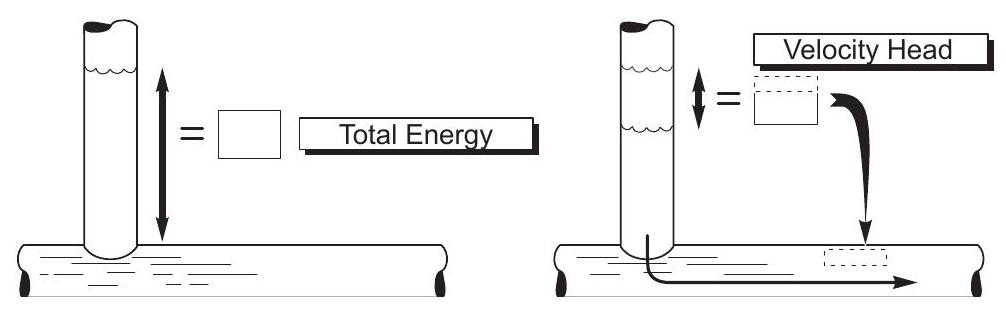
\includegraphics[scale=0.25]{2022_11_03_65aa625ded296bdfd01fg-20}
\end{center}
\textbf{Total Dynamic Head: }  Total dynamic head (TDH) is a theoretical distance. It is the static head, velocity head and headloss required to get the water from one point to another.

The horsepower output of an electric motor is directly reflected to the amperage that the motor draws. Any increase in horsepower requirements will give a corresponding increase in amperage.

\textbf{Cavitation: }  Cavitation in pumps is the rapid creation and subsequent collapse of air bubbles occuring as a result of the inlet pressure falling below the design inlet pressure or when the pump is operating at a flow rate higher than the design flow rate. This collapse of the air bubbles typically manifests as a pinging or crackling noise.  Cavitation is undesirable because it can damage the impeller, cause noise and vibration, and decrease pump efficiency.

\begin{figure}[h]
\begin{center}
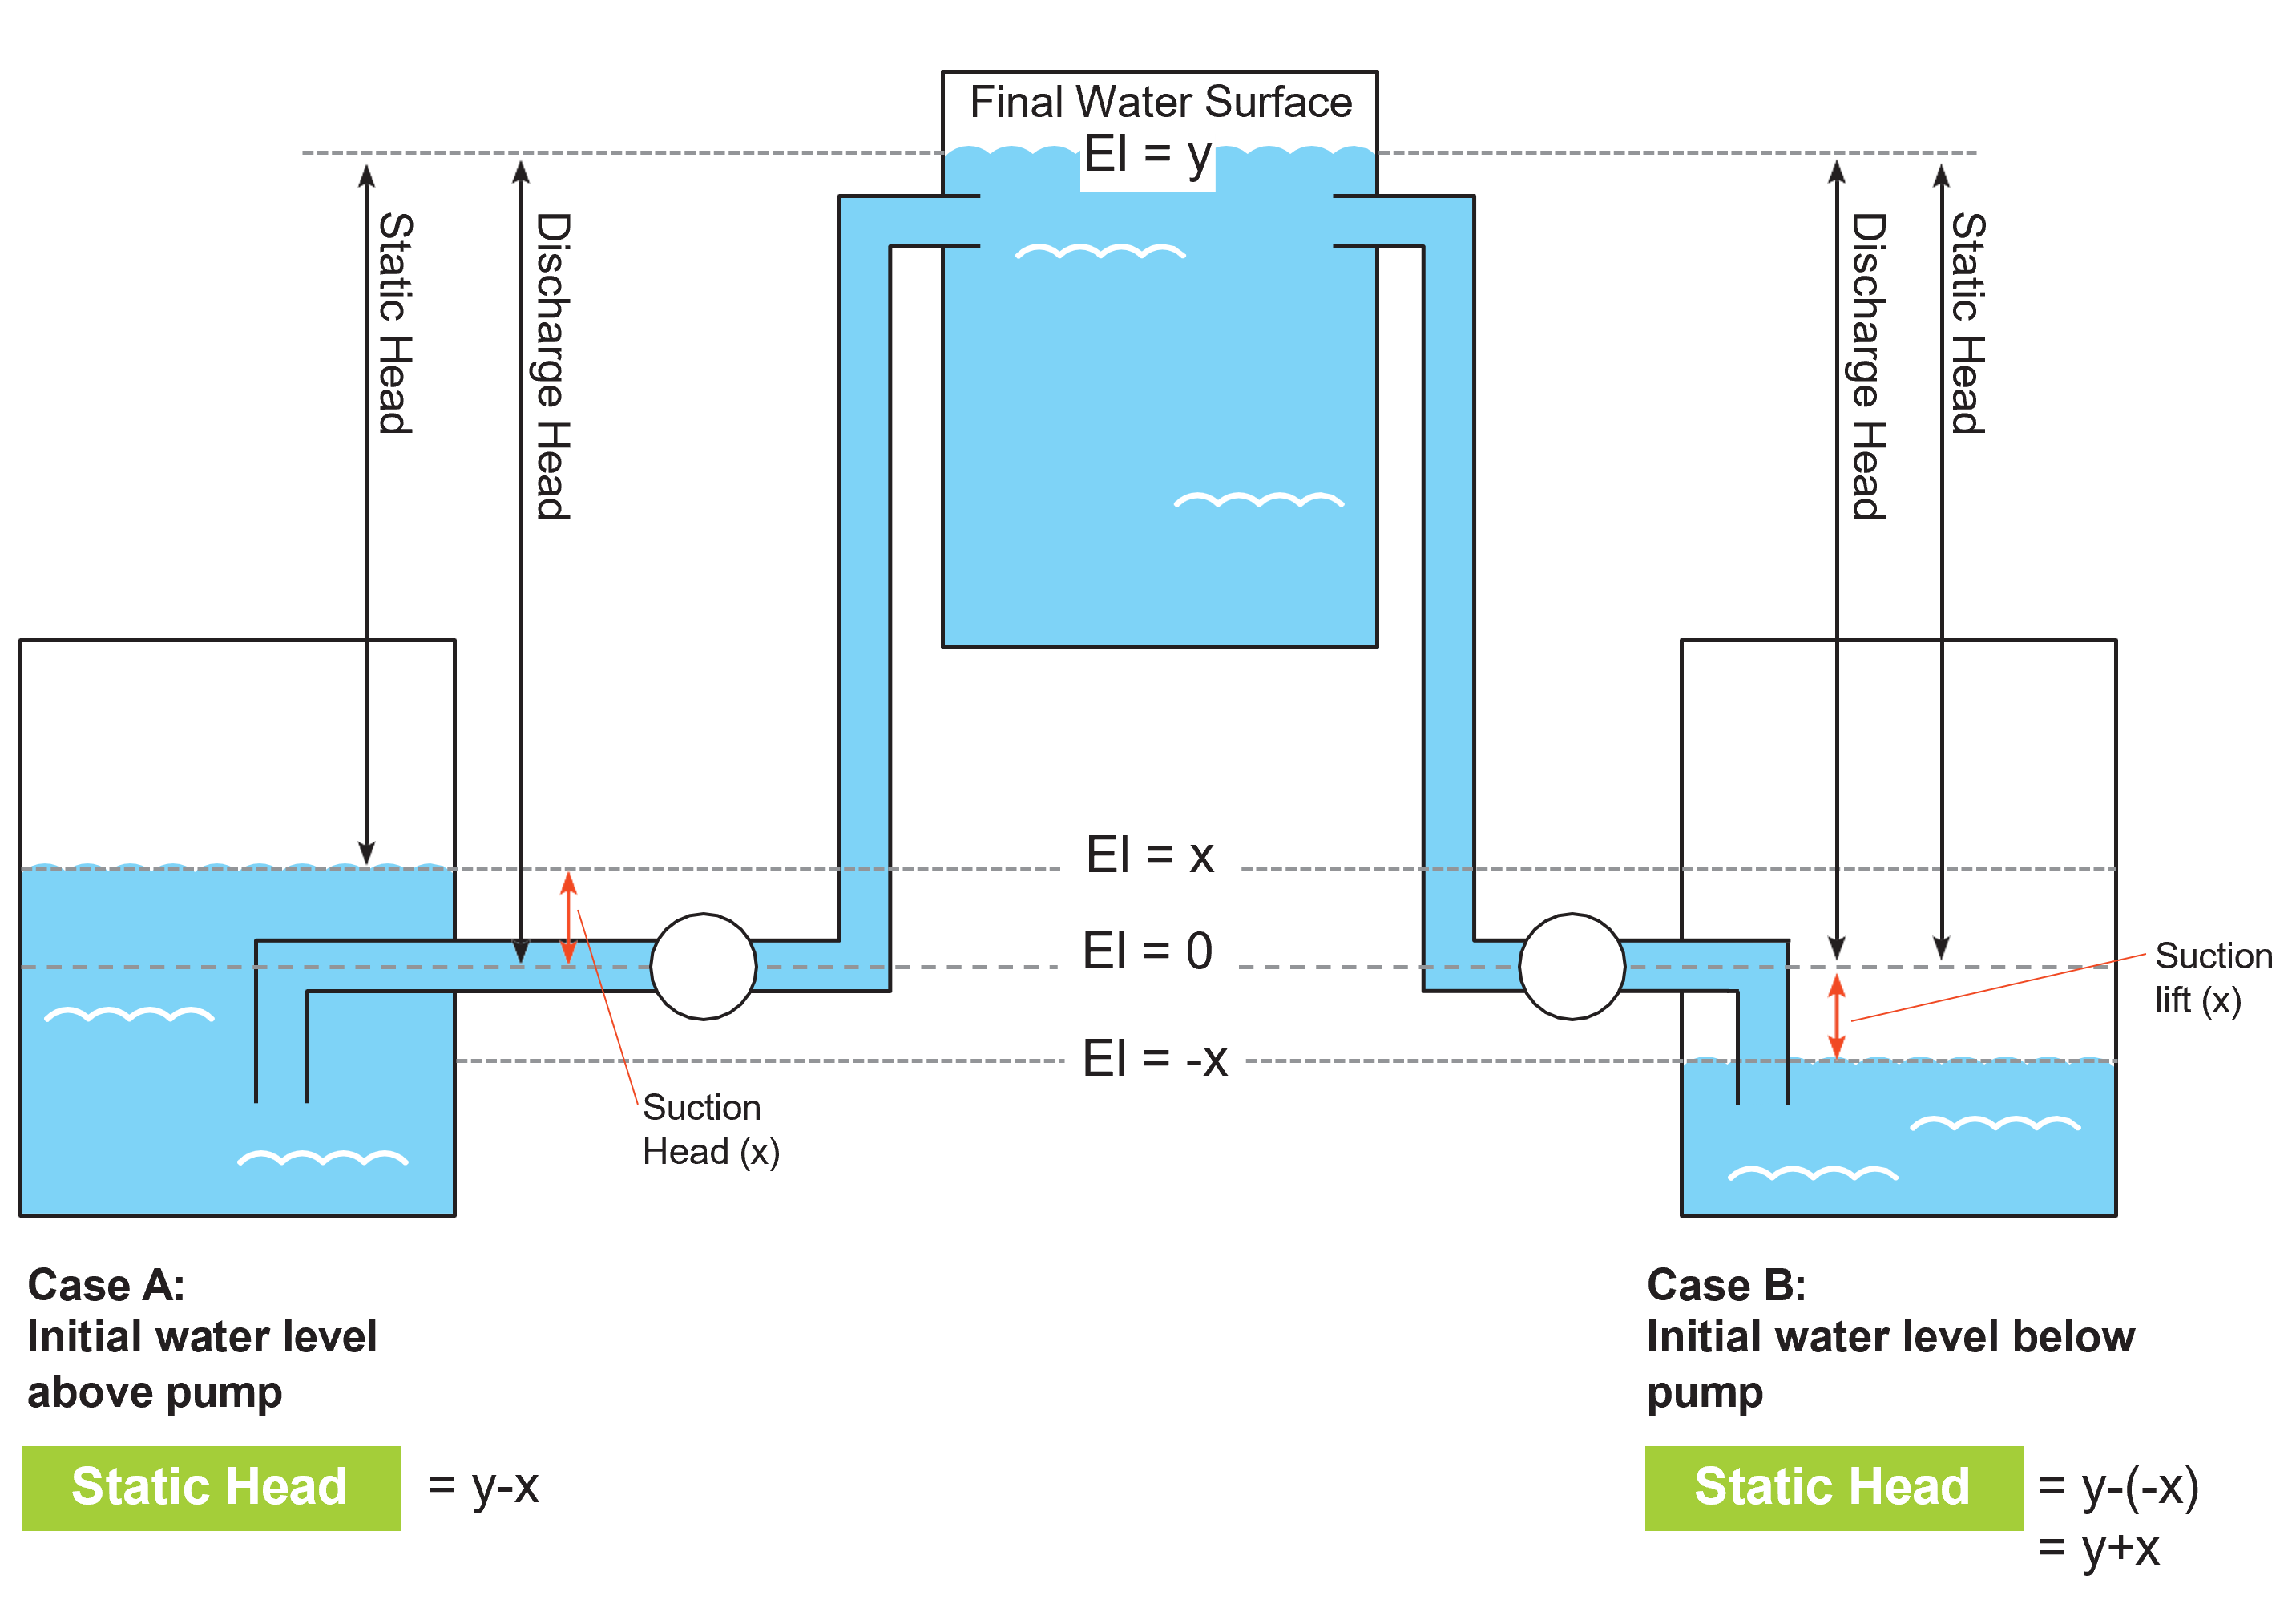
\includegraphics[scale=0.6]{CalculatingStaticHead}\\
\includegraphics[scale=0.6]{PumpHead}\\
\end{center}
\end{figure}

\section{Pumping Rate Calculations}\index{Pumping Rate Calculations}
\begin{itemize}
\item \texthl{For calculating volume pumped given the pump flow rate:} Multiply the pump flow rate by the time interval\\
\textbf{Make sure:}
\begin{itemize}
\item The time units - in the given time interval and in the pump flow rate match
\end{itemize}
\item \texthl{For calculating time to pump a certain volume:}
\begin{enumerate}[Step 1.]
\item Calculate the total volume pumped
\item Divide the total volume by the pump flow rate
\end{enumerate}
\textbf{Make sure:}
\begin{itemize}
\item The volume units - in the volume that needs to be pumped and in the pump flow rate match
\item The time unit in the pump flow rate needs to be converted to the time unit that you need the answer in
\end{itemize}
\end{itemize}
% \end{enumerate}

\section{Power Requirements for Pumping}\index{Power Requirements for Pumping}
\begin{center}
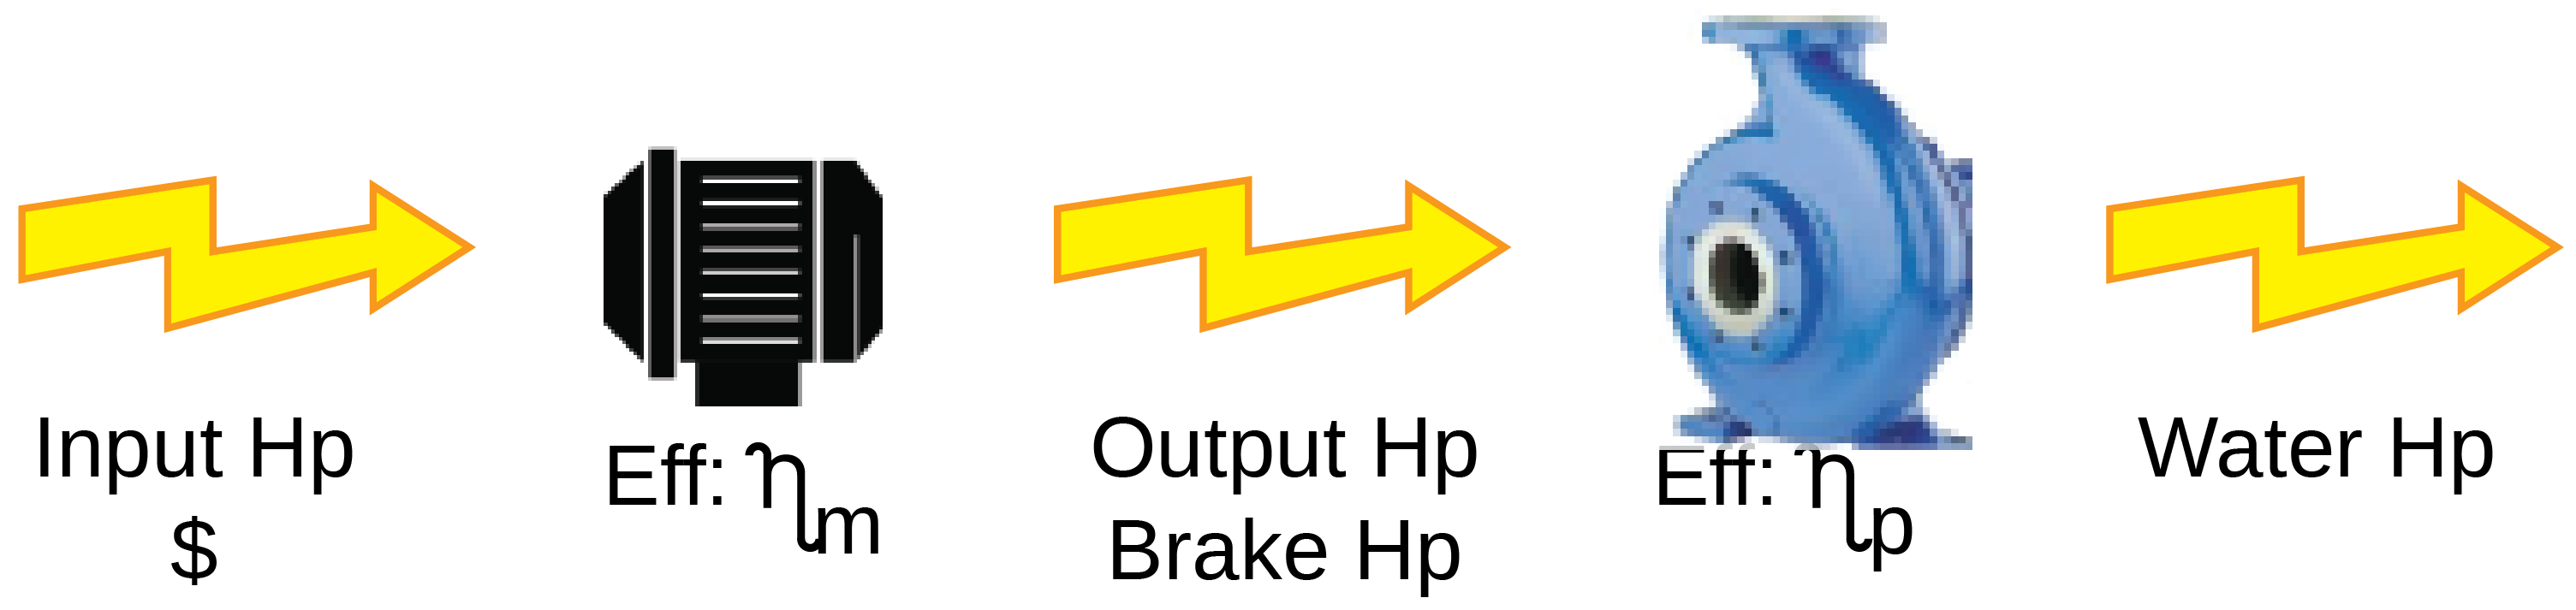
\includegraphics[scale=0.12]{PumpProblem}\\
\end{center}
Where:\\
\begin{itemize}
\item \textbf{Input Hp} is the input power to the motor which produces the \textbf{Output Hp or Brake Hp} - the mechanical power which runs the pump.  
\item The ratio of Output Hp and Input Hp is the motor efficiency - $\eta_m$.
\item The Output Hp is the input power (Brake Hp) to the pump to pump the water.
\item Water Hp is the rate of energy transferred to the water being pumped and can be calculated by the formula:\\
$$\dfrac{\mathrm{H \enspace - \enspace Head \enspace of \enspace water \enspace (ft) \enspace * \enspace Q \enspace - \enspace Flow \enspace (GPM)}}{3,960 \enspace \mathrm{(Conversion \enspace factor \enspace for \enspace converting \enspace GPM-ft \enspace to \enspace Hp)}}$$
\item The ratio of Output Hp and Water Hp is the pump efficiency - $\eta_p$.
\end{itemize}


\section{Summary of conversions and formulas}\index{Summary of conversions and formulas}

Total dynamic head = Friction head + Static head\\
\vspace{0.3cm}
$1Hp=0.746kW$\\
\vspace{0.3cm}
$1Hp=\dfrac{33,000 \enspace ft-lb}{min}$\\
\vspace{0.3cm}
$1Hp=3,960 \enspace GPM-ft$\\
\vspace{0.3cm}
$1psi=2.31ft$\\
\vspace{0.3cm}
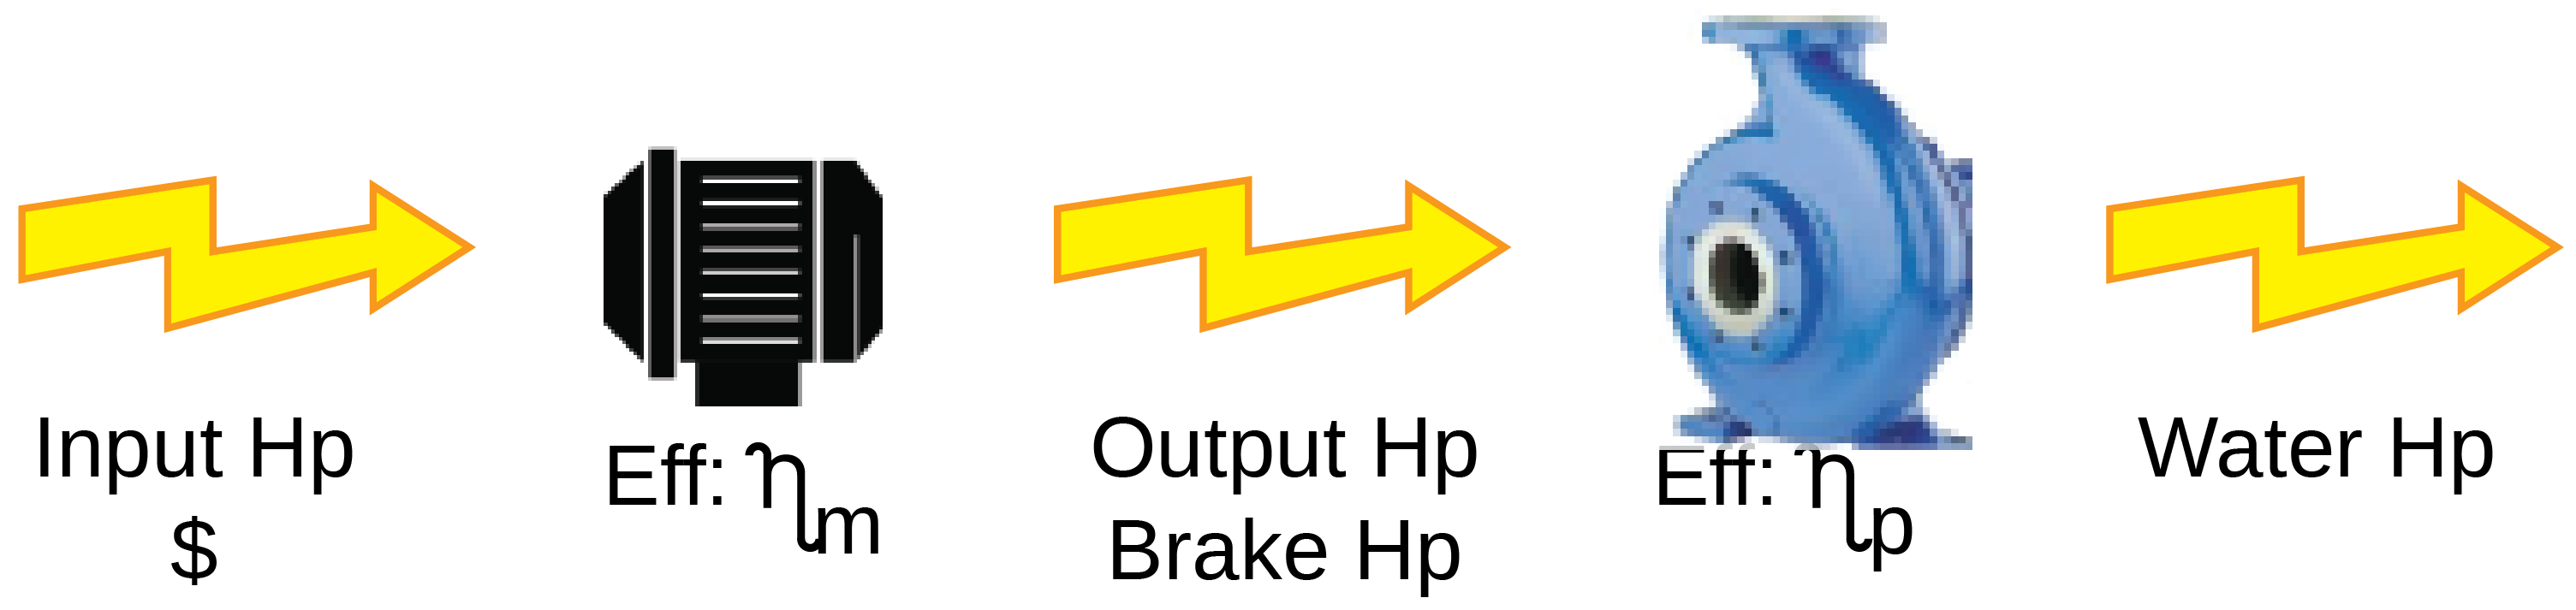
\includegraphics[scale=0.08]{PumpProblem}\\
\vspace{0.3cm}
$Water \enspace Hp \enspace = \enspace Flow \enspace *  \enspace Head$\\
\vspace{0.3cm}
$Brake  \enspace Hp \enspace = \enspace Input \enspace Hp*Motor \enspace efficiency$\\
\vspace{0.3cm}
$Water  \enspace Hp \enspace = \enspace Brake \enspace Hp \enspace * \enspace Pump  \enspace efficiency,  \enspace and$\\
\vspace{0.3cm}
$\implies Water  \enspace  Hp \enspace = \enspace Input  \enspace  Hp \enspace * \enspace Motor  \enspace efficiency \enspace * \enspace Pump  \enspace efficiency$\\

\newpage
\thispagestyle{empty}
% \begin{landscape}
% 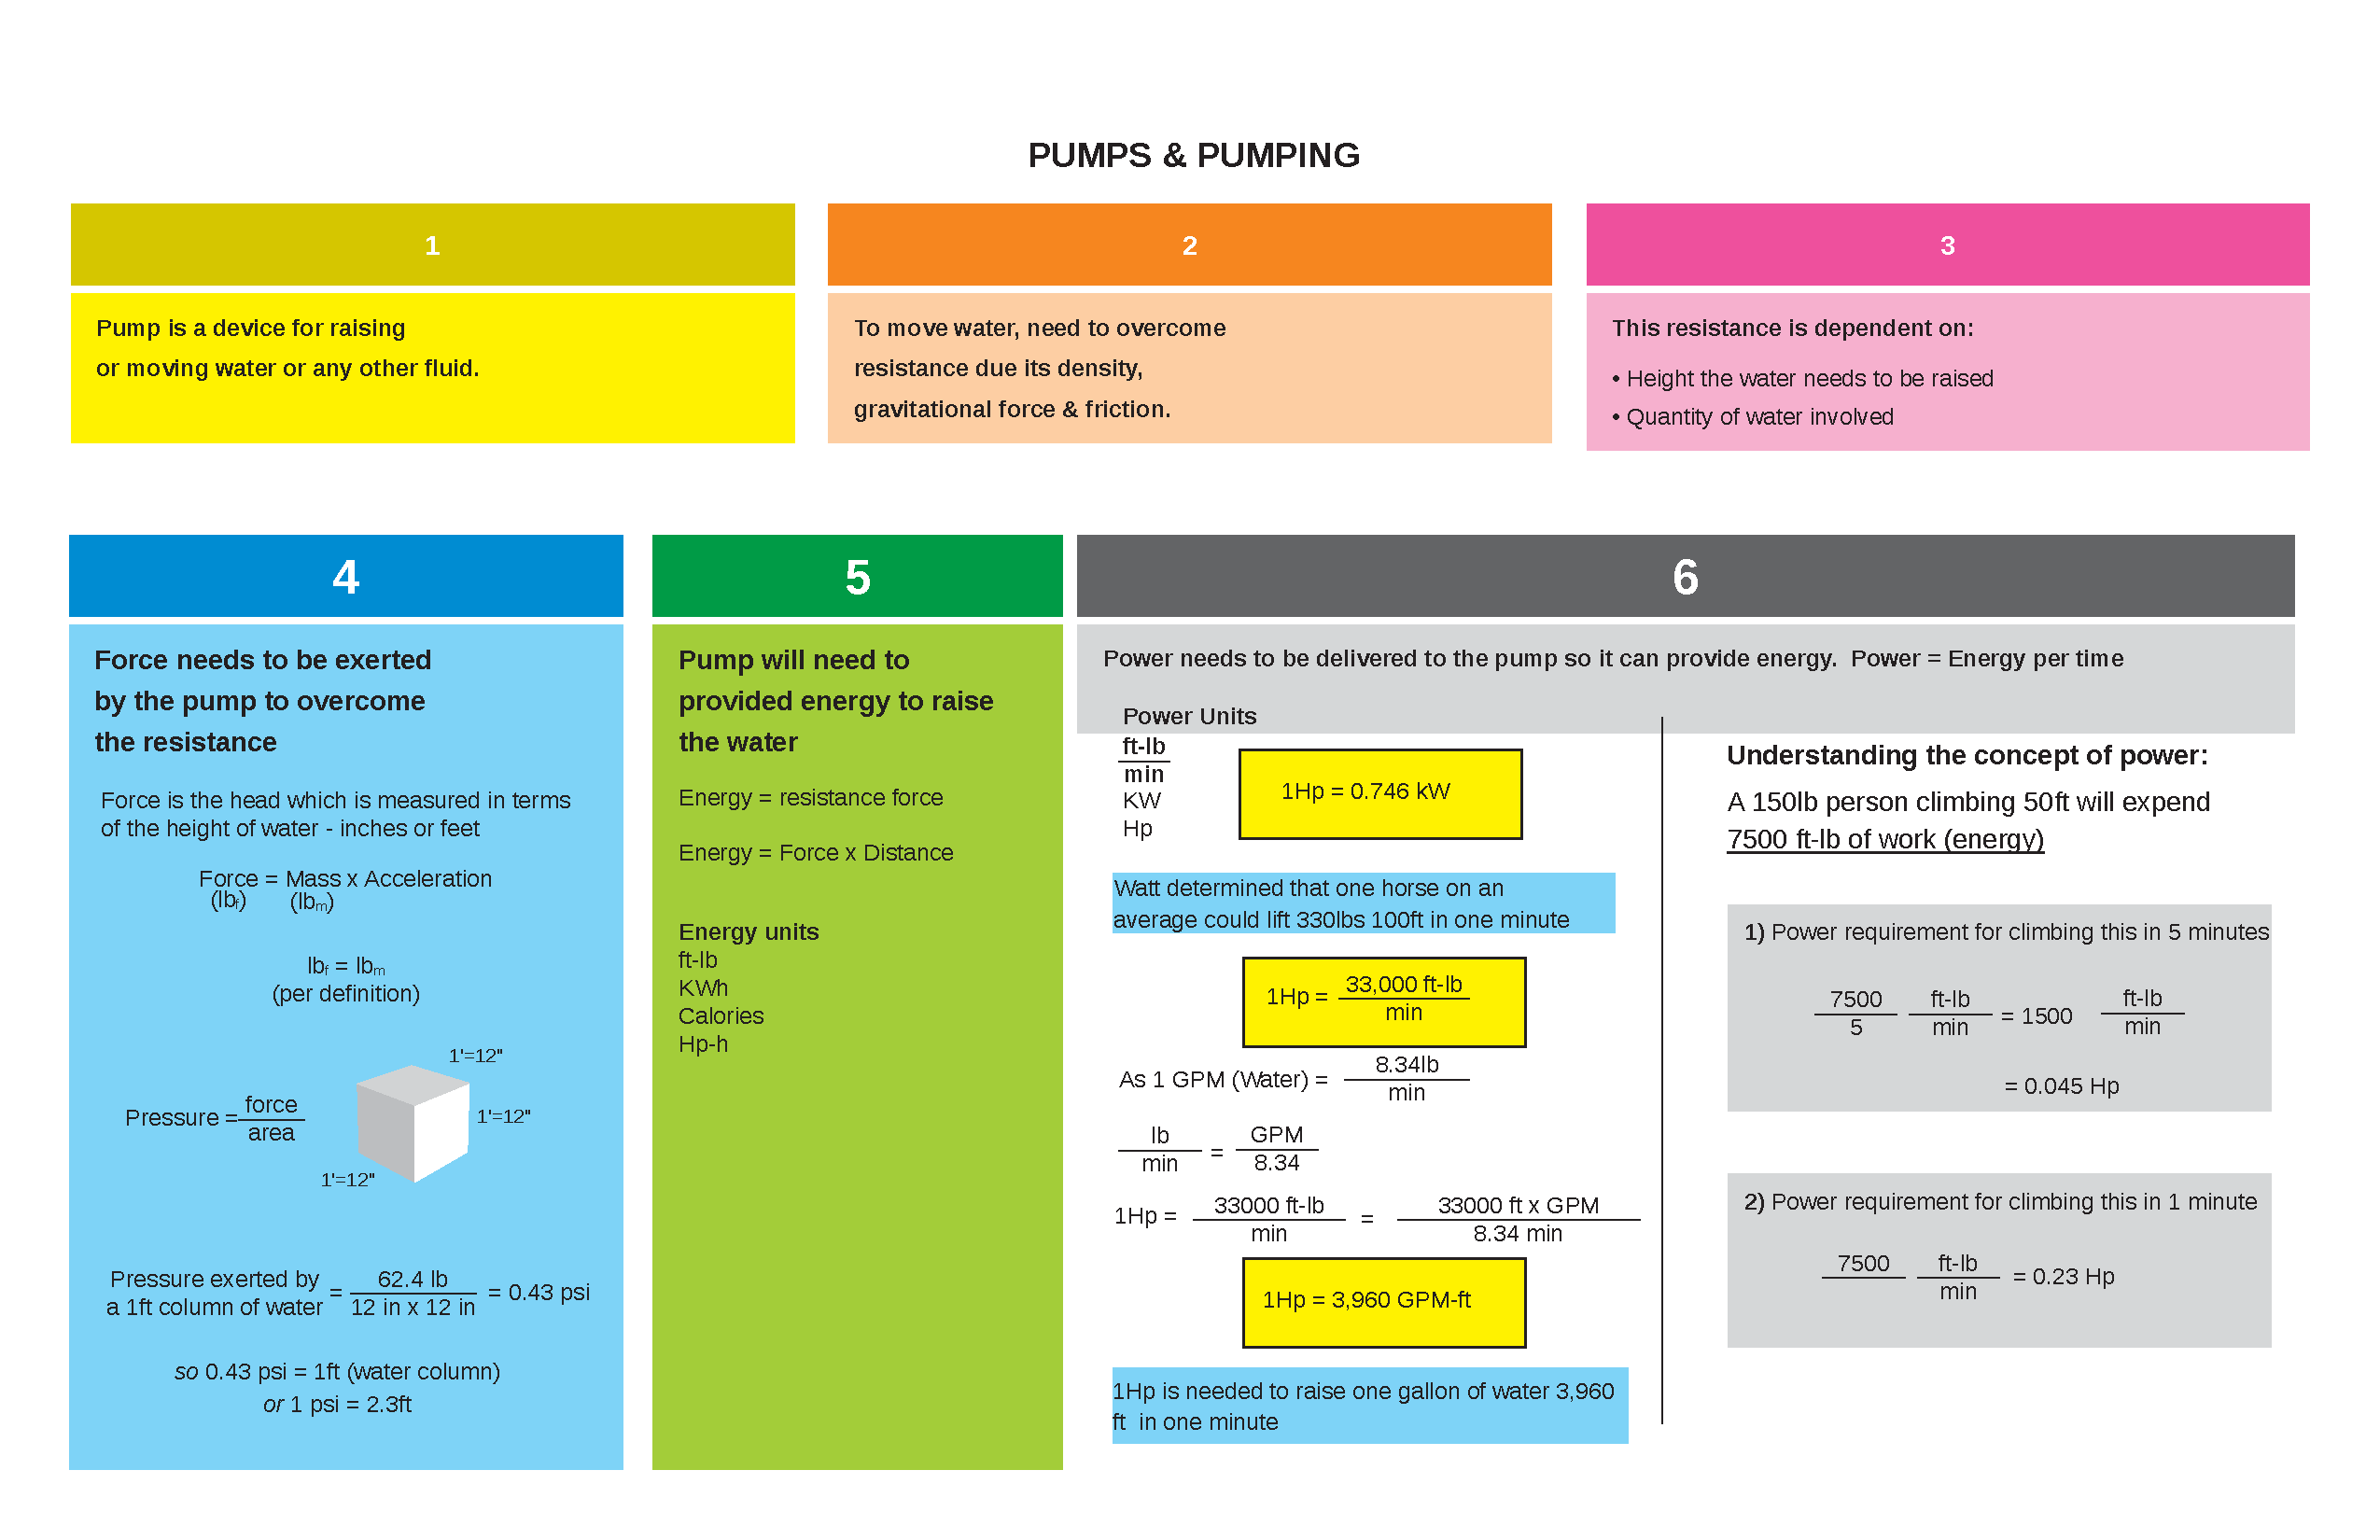
\includegraphics[scale=0.52]{PumpsandPumpingR1_01.pdf}
% \end{landscape}
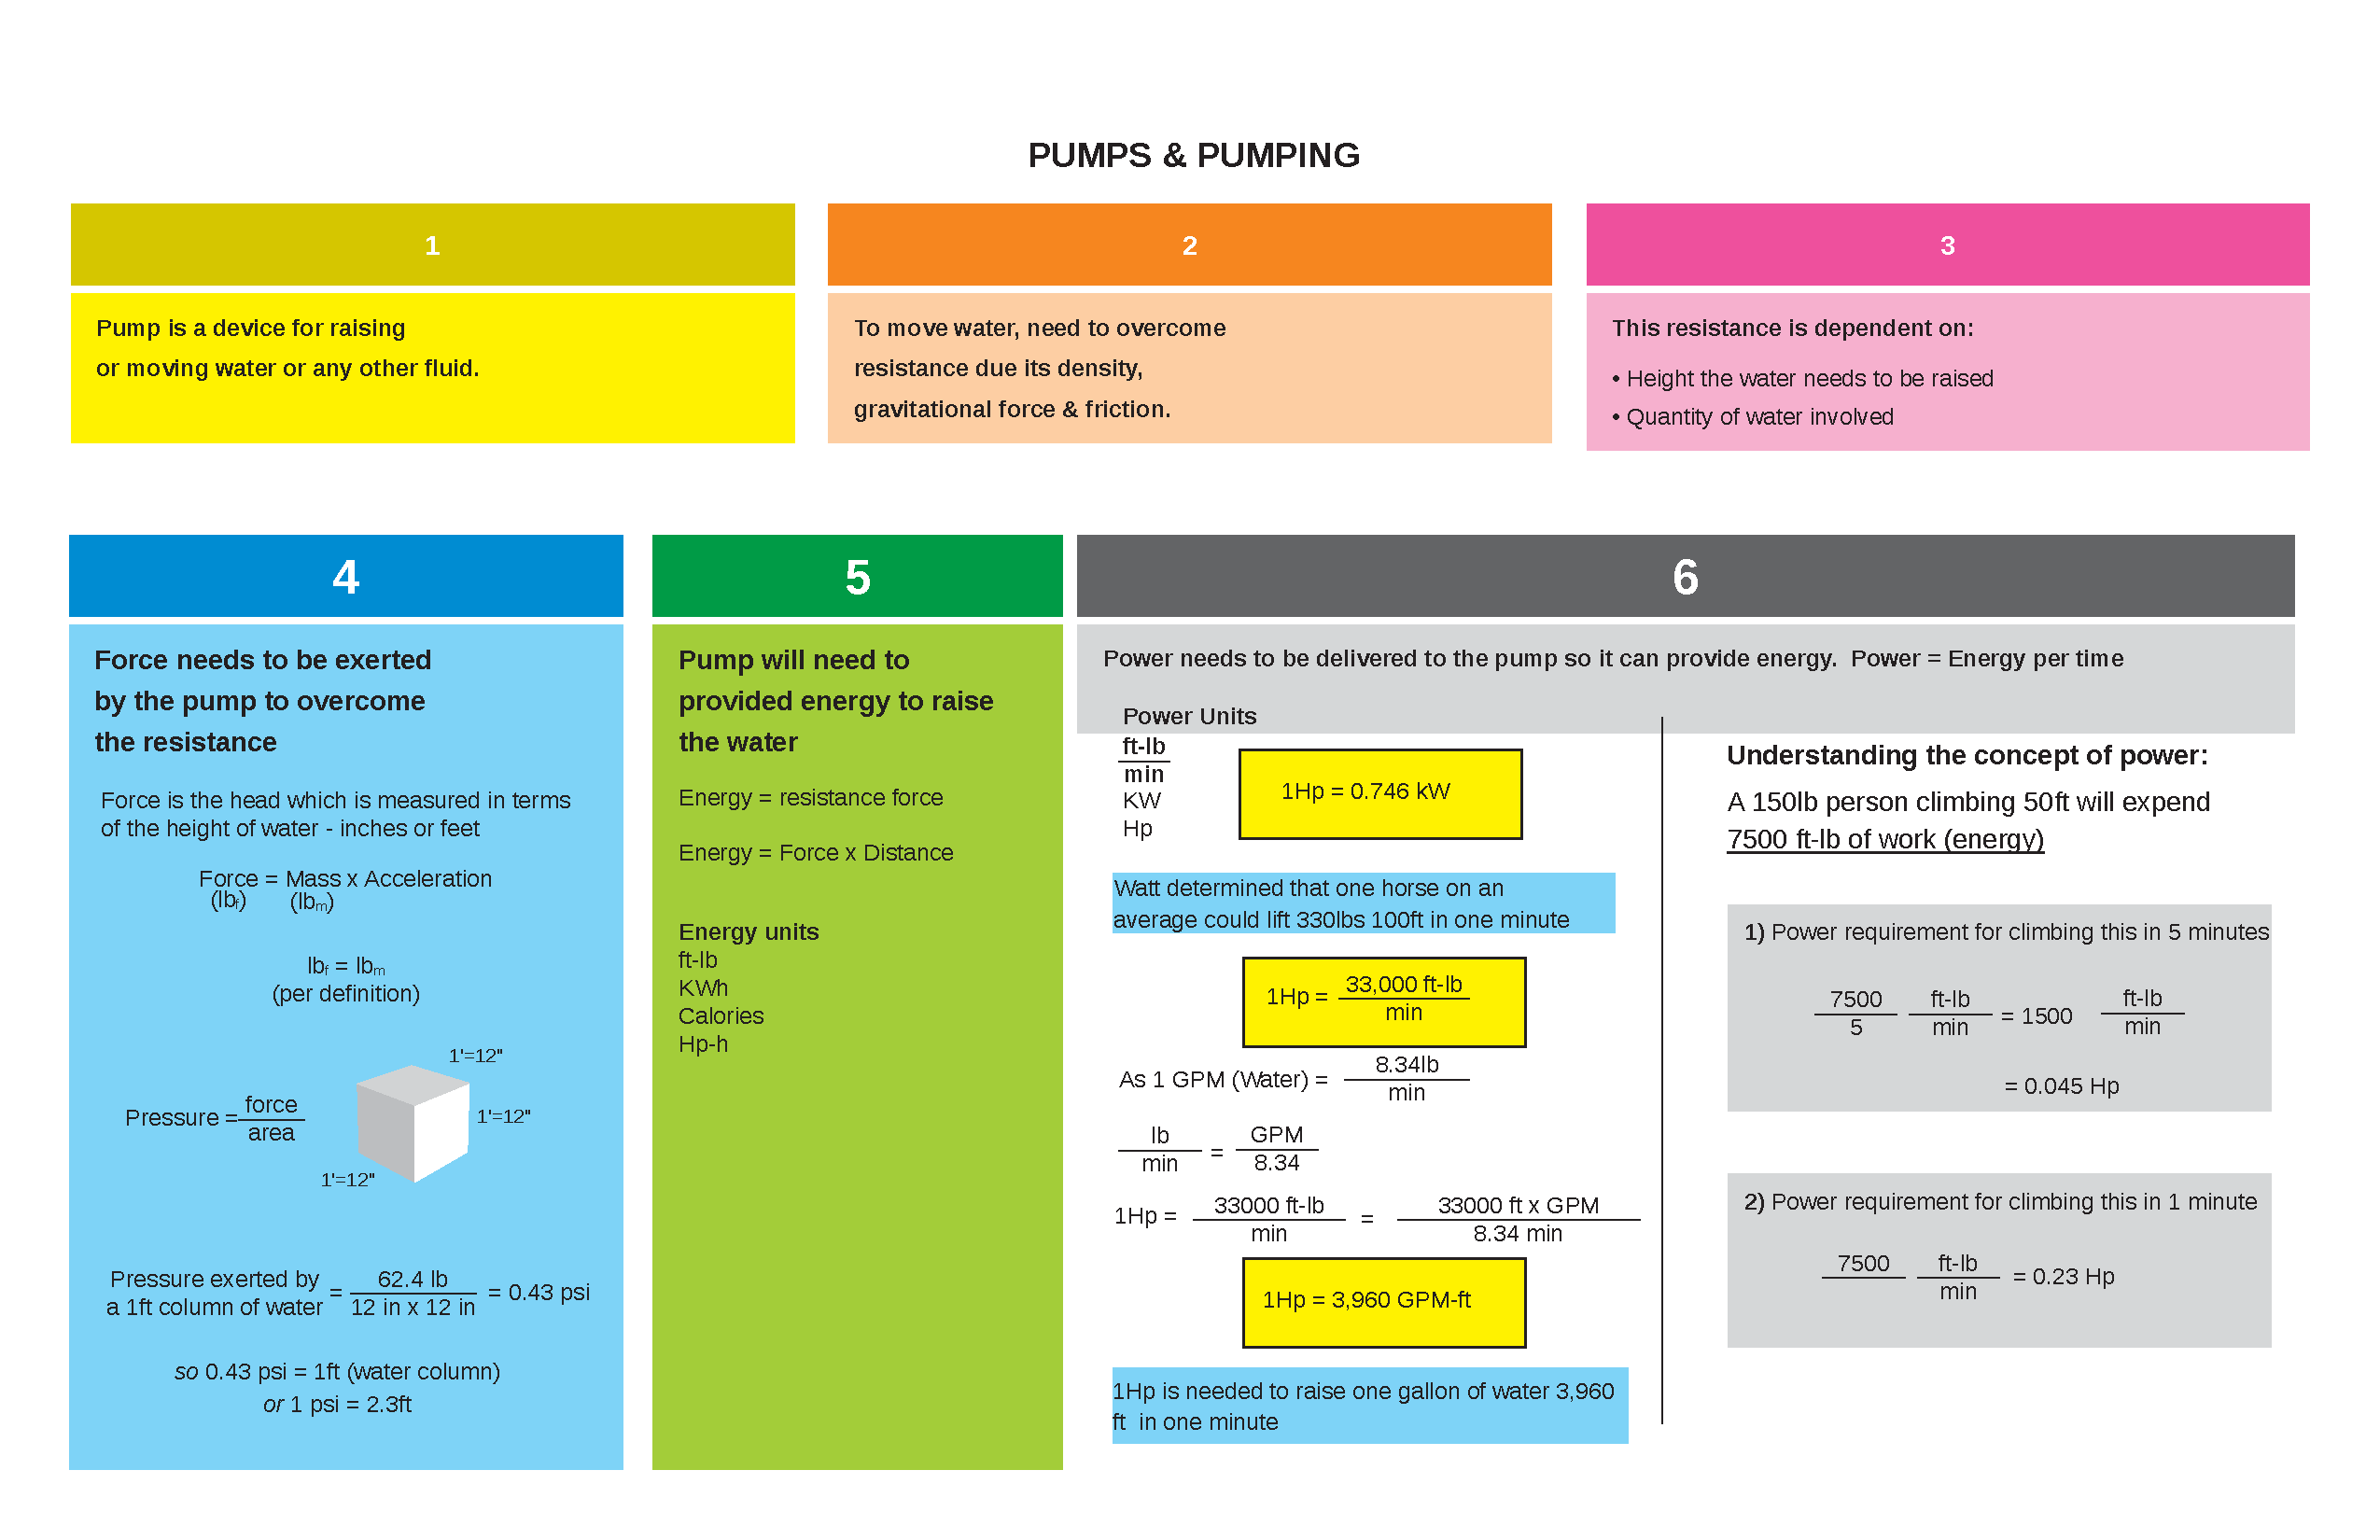
\includepdf[landscape=true]{PumpsandPumpingR1_01.pdf}
\newpage

\thispagestyle{empty}
% \begin{landscape}
% 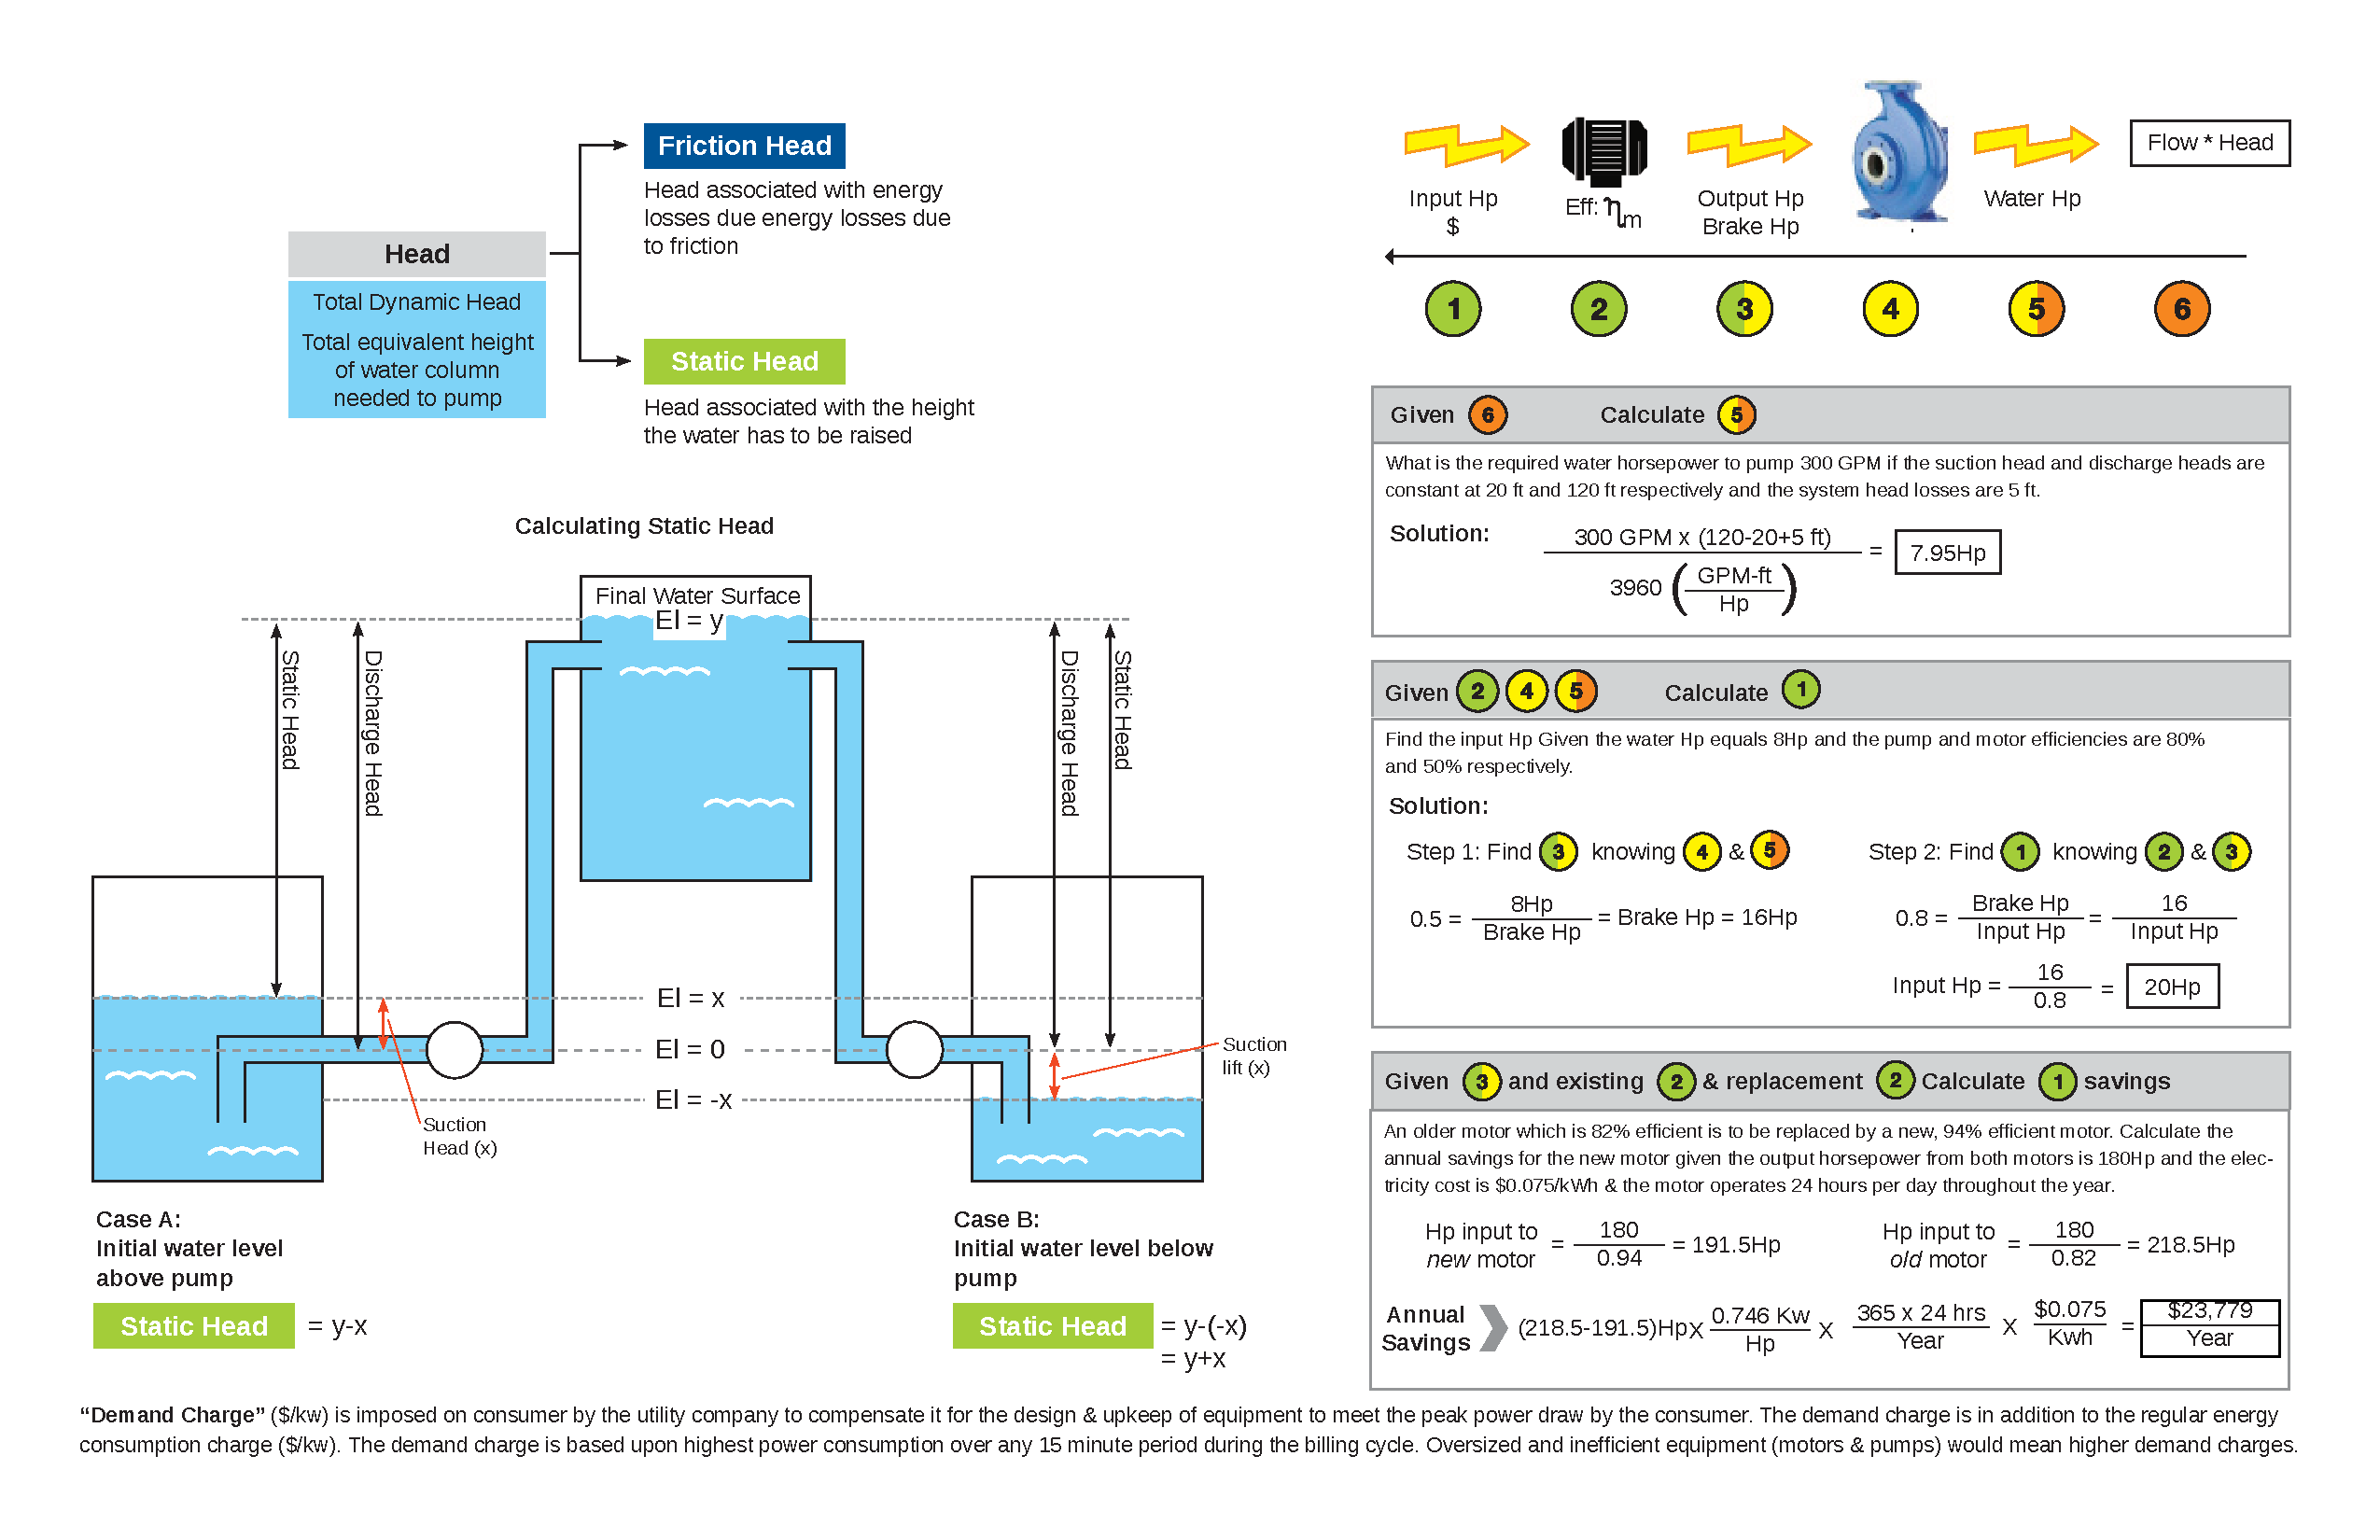
\includegraphics[scale=0.52]{PumpsandPumpingR1_02.pdf}
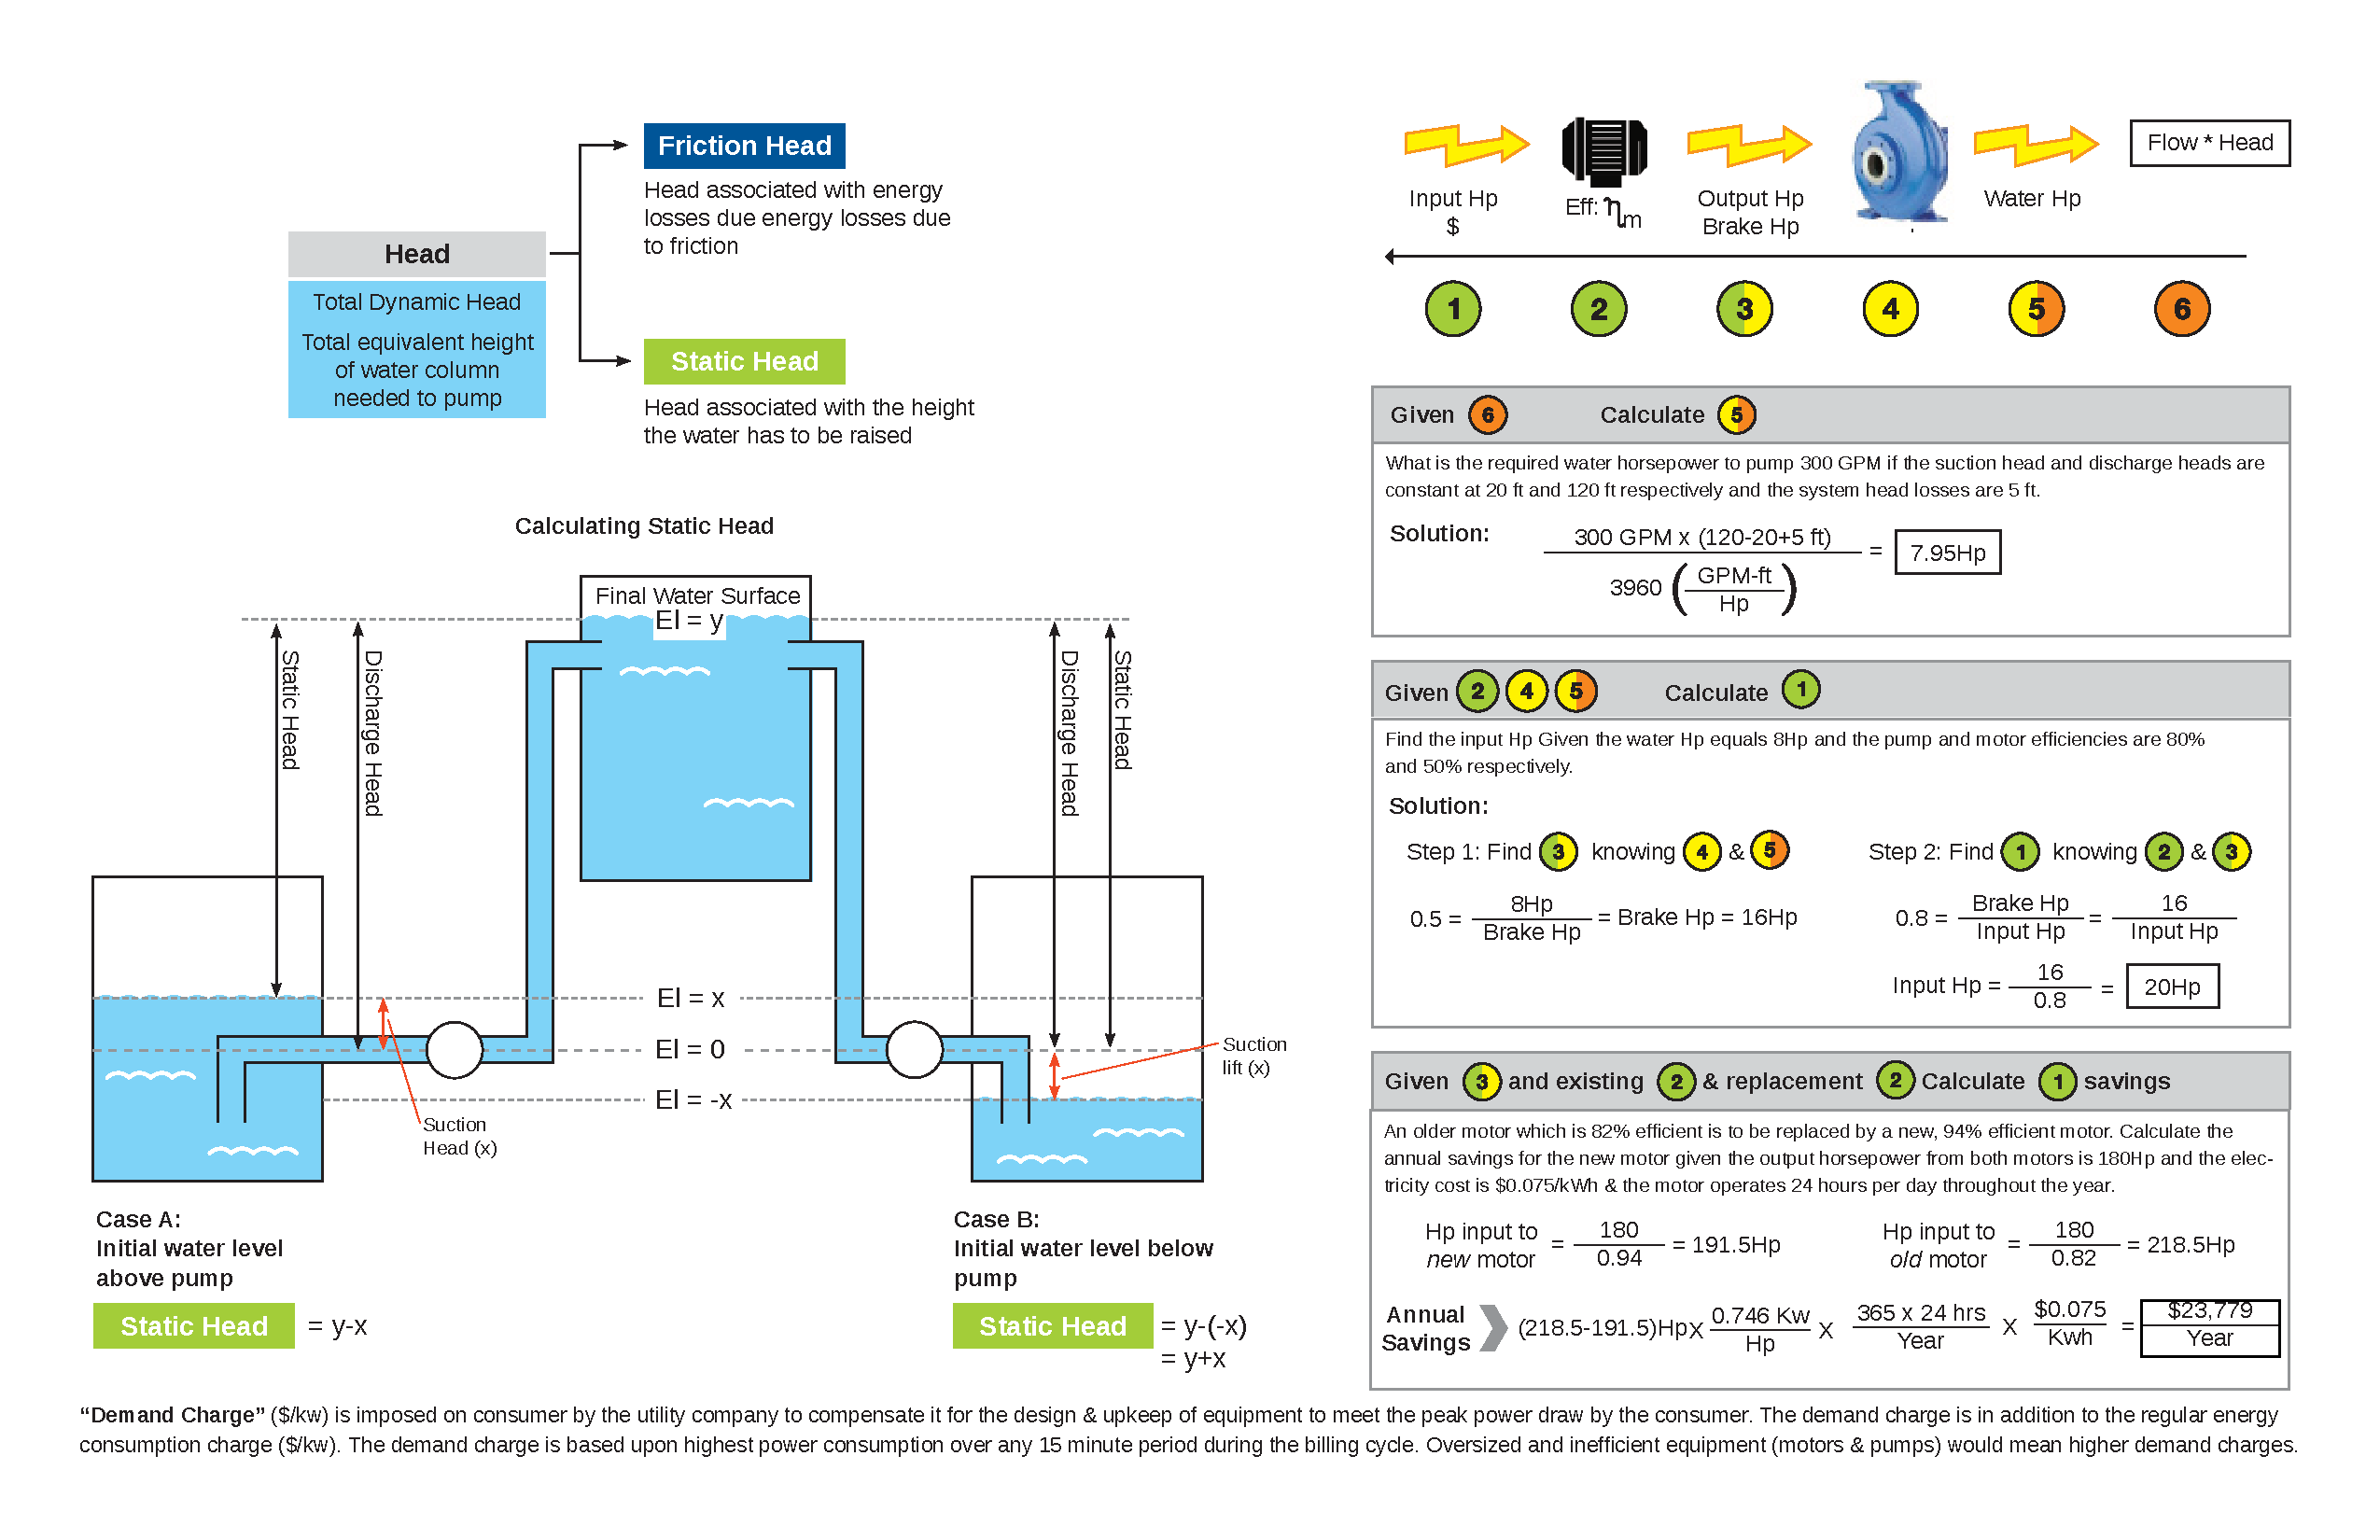
\includepdf[landscape=true]{PumpsandPumpingR1_02.pdf}
% \end{landscape}
\newpage



\newpage
\begin{tcolorbox}[breakable, enhanced,
colframe=blue!25,
colback=blue!10,
coltitle=blue!20!black,  
title= Chapter Assessment]

\begin{enumerate}
\item  A positive displacement pump should be started up with the discharge valve closed in order to avoid any problems with "air lock". 

a. True \\
b. False 


\item  Brake horse power is the input power to the motor 

a. True \\
b. False 


\item  Cost of electrical usage for pumps is based upon kilowatt per hour 

a. True \\
b. False 


\item  A centrifugal pump can be used to pump sludge. 

a. True \\
b. False 


\item  Variable speed sludge pumps may be used to keep the density of the sludge nearly constant. 

a. True \\
b. False

\item  What is the vertical distance between the elevation of the free water surface at the suction and that of the free water surface at the discharge of a pump called?\\
a.  Discharge head.\\
b.  Dynamic head.\\
c.  Velocity head.\\
d. Static head.\\

\item Static suction head plus friction suction head plus static discharge head plus friction discharge head is a pump's\\
a. Pump curve\\
b. Operating pressure\\
c. Efficiency\\
d. Total dynamic head\\
e. Velocity head\\

\end{enumerate}
\end{tcolorbox}